
Put your Experimental results
\section{Testing Frame Construction(FrameObj)}
%Rebecca
% not sure how much of this le will go over...so super brief here
An easy way of being able to integrate with the other teams seemed to be through the creation of a class, FrameObj, which would not only provide the other modules with a means of creating a frame but a list of properties that could be called for easy debugging. There are two ways that an instance of the class FrameObj could be constructed,  from the basic requirements of the frame (Frame type, Sender ID number , Receiver ID number, and Data) or from the bits of data that make up a frame.

4 sections of testing that done to frame object. 

section 1 tests the ways we can make an invalid frame








\section{End-to-End Local Machine Testing }
%Renato
The test of the implementation of the end to end communication.
Based on proposal of final design project \cite{cdproj}, there
are six case to be tested in the end to end communication
\begin{enumerate}
  \item Extra-cellular communications between UEs
  \begin{enumerate}
    \item US1 $\rightarrow$ BS1 $\rightarrow$ BS2 $\rightarrow$ US3
    \item US3 $\rightarrow$ BS2 $\rightarrow$ BS1 $\rightarrow$ US1
		\item US2 $\rightarrow$ BS1 $\rightarrow$ BS2 $\rightarrow$ US3
		\item US3 $\rightarrow$ BS2 $\rightarrow$ BS1 $\rightarrow$ US2
  \end{enumerate}
  \item Intra-cellular communications between UEs
	  \begin{enumerate}
    \item US1 $\rightarrow$ BS1 $\rightarrow$ US2
    \item US2 $\rightarrow$ BS1 $\rightarrow$ US1
	\end{enumerate}
\end{enumerate}

The figure \ref{fig:endendDiagram} show how the whole MATLAB code is organized to test all the cased described in this section.
The send and received part maps each path of information lie UE 1 to BS1 as a channel . It more logical representation that to a physical channel to the end
to end implementation in the final integration.
The routing used was just a siwtch case based on picture of proposed network in \cite{cdproj}.
The send and received is a recursive function that call it self based with parameters changed for the routing.
One examples is shown in listing \ref{sendReceiveExample} show how inside a channel based on direction how it will resend the message or exit the the function based on the destination.
\lstset{caption={Code examples how to verify the CRC and create the ACK message back to sender},label=sendReceiveExample}
\lstinputlisting{code/sendReceiveExample.M}

The listing \ref{crcVerification} is a examples how the receveive UE in the figure \ref{fig:endendDiagram} verify the CRC and create the new frame to send back.
It procedure is important because it need to be done in the integration with other team that need to use the frameObj.     

\lstset{caption={Code examples how to verify the CRC and create the ACK message back to sender},label=crcVerification}
\lstinputlisting{code/crcVerification.M}



\begin{figure}[ht]
    \centering
    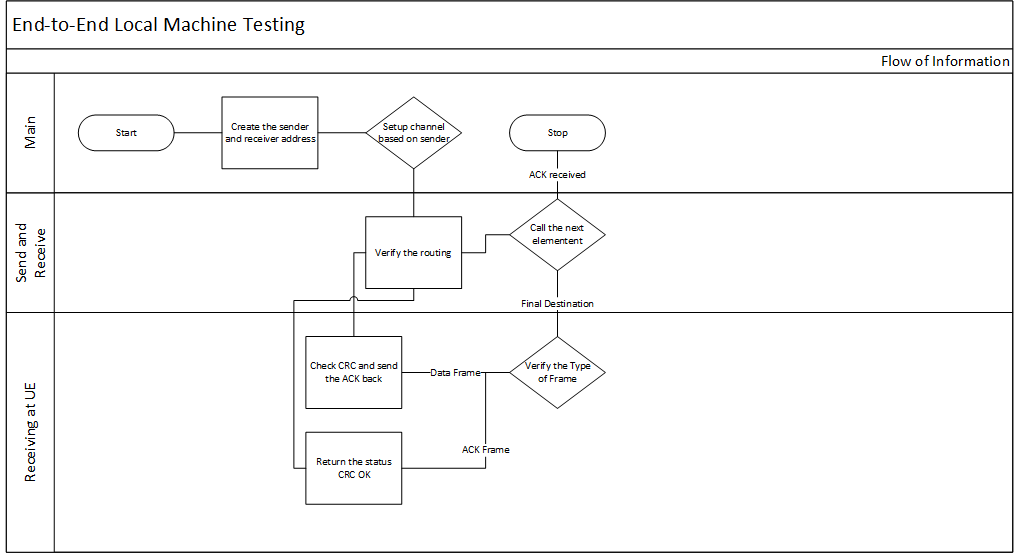
\includegraphics[width=0.8\textwidth]{flowEndtoEnd.PNG}
    \caption{Diagram of the flow of information to test the end to end in Matlab for the team 6 proposed protocol}
    \label{fig:endendDiagram}
\end{figure} 

\section{Transmitting and receiving over the air}
%Renato
The frame object need to be tested over the air to check if it behaves as expected in our simulation. 
It was tested using two diffetne physical layer. 
\subsection{Using lab2 physical layer}
The first test was using a very straight forward approach. We just replaced the 'hello world' message in the Lab 2 
simulating model to add the frame object with a message 'Hi', so it can near the orginal size of the message.

\begin{table}[ht]
	\centering
		\begin{tabular}{| c | c | }
		\hline                       
		Frame Type UE & Number Received\\
		\hline
			ACK & 2\\
			DATA & 102\\
			corrupt DATA & 2\\
			INVALID & 3466\\
			other & 0\\
		\hline
		\end{tabular}
	\caption{Table of frames received with poor transmission quality and a small hamming distance between frame types}
	\label{tab:2ACK}
\end{table}

\begin{table}[ht]
	\centering
		\begin{tabular}{| c | c | }
		\hline                       
		Frame Type & Number Received\\
		\hline
			ACK & 0\\
			DATA & 165\\
			corrupt DATA & 4\\
			INVALID & 3559\\
			other & 0\\
		\hline
		\end{tabular}
	\caption{Table of frames received with poor transmission quality and a larger hamming distance between frame types}
	\label{tab:0ACK}
\end{table}

\subsection{Using Team 4 physical layer}

